\documentclass[a4paper,12pt]{article}
\usepackage{graphicx}
\usepackage[left=30mm, right=30mm, top=30mm, bottom=35mm]{geometry}
\usepackage{amsmath}
\usepackage{siunitx}
\usepackage{booktabs}
\usepackage{fancyhdr}
\usepackage{url}
\pagestyle{fancy}
%-------------------------------------------------------------------------------
\lhead{\textbf{Spring 2020}}
\rhead{\textbf{CE394M Advanced Analysis in Geotechnical Engineering}}
\cfoot{\thepage}
%-------------------------------------------------------------------------------

\begin{document}
\begin{centering}
	\textbf{
		Assignment 01: Finite Element Analysis\\
		Assigned: 28th January 2020\\
		Due: 03rd February 2020 at 10AM\\
	}
\end{centering}

\vspace{1em}
 
Perform short-term finite element analyses of the slope from Assignment 00 using the Optum G2 software. 

\begin{itemize}
	\item Plot the magnitude of displacement from the analyses
	\item Compare the effect of Element type, element size and mesh adaptivity
	\item For mesh adaptivity yes/no compare the results only for 15-noded Gauss element with 1000 elements.
	\item List as many unresolved questions you may have regarding the analyses.
\end{itemize}

Please use the following configuration for the FE analyses. 

\begin{table}[!h]
	\centering
	\begin{tabular}{ll}
		\toprule
		\textbf{Description}     & \textbf{Values} \\
		\midrule
		Analysis type & Elastoplastic\\
		Element types  &   6-noded and 15-noded Gauss\\
		Element sizes   & 100, 500, 1000, 2500    \\
		Mesh adaptivity & No\\
		Load steps & 10 \\
		\bottomrule
	\end{tabular}
\end{table}

\begin{figure}[!h]
	\centering
	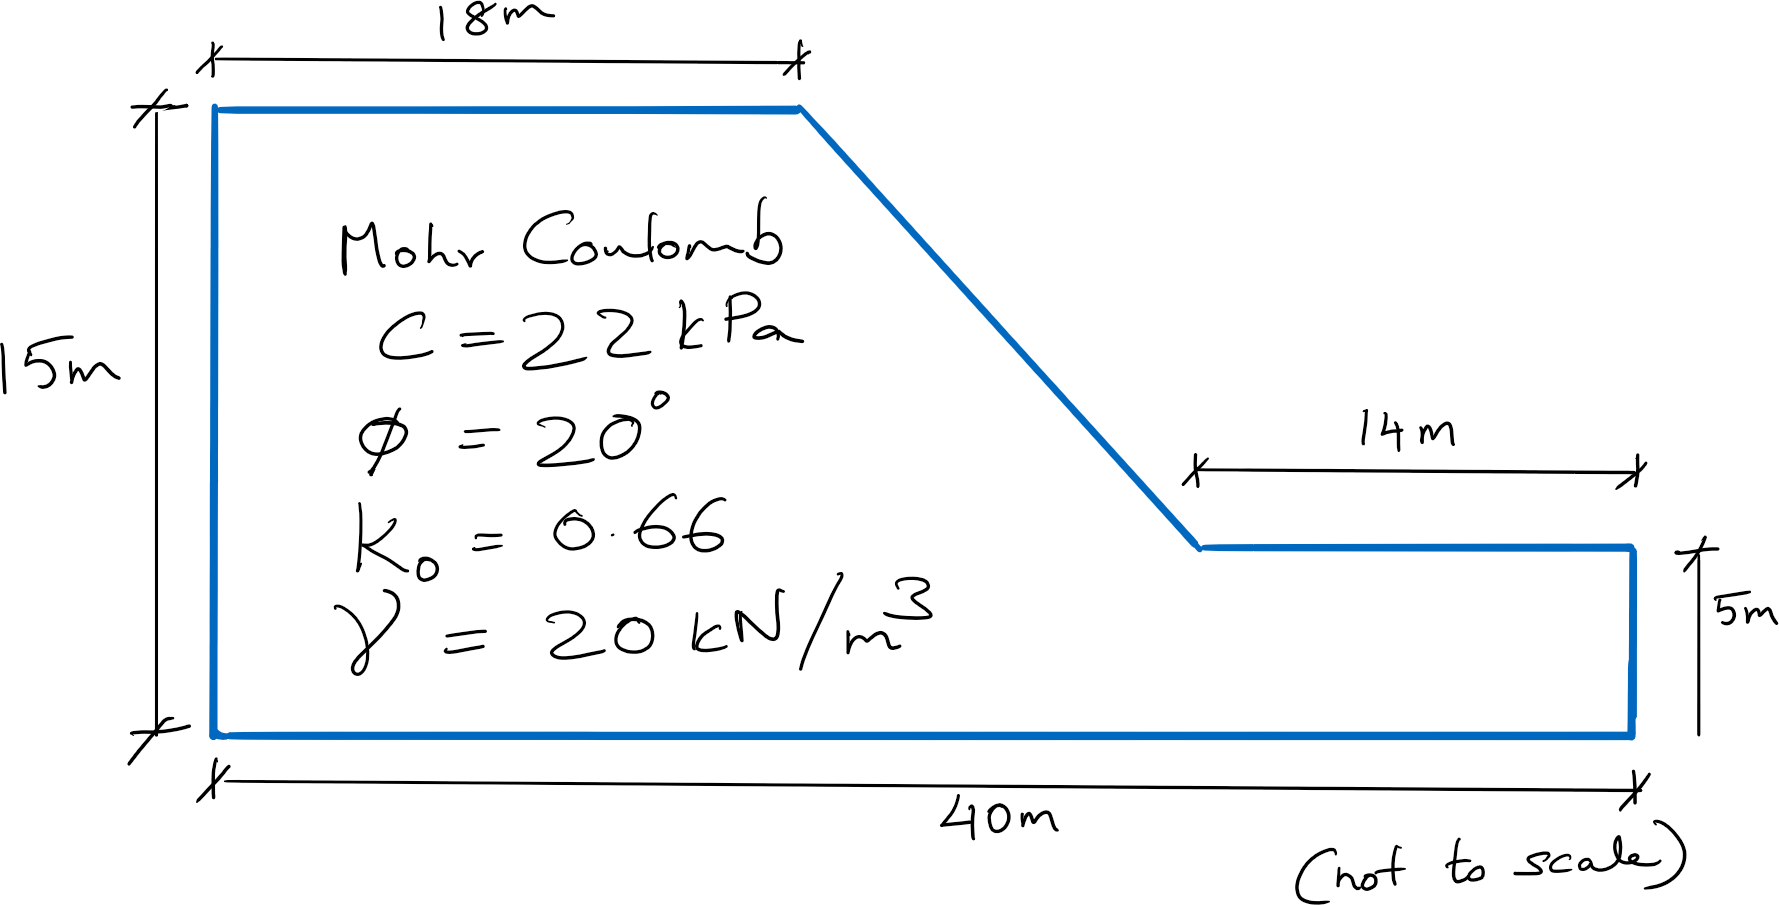
\includegraphics[width=0.75\textwidth]{figs/slope.png}
\end{figure}


	
\end{document}

